%\documentclass[spanish]{beamer}
\documentclass{beamer}
\usepackage{pgf,pgfpages}
%\pgfpagesuselayout{4 on 1}[letterpaper,landscape,border shrink=0.5in]
\usepackage{algorithm,algorithmic}
%\usepackage{algorithm,algorithmicx}
%\usepackage[noend]{algpseudocode}
\usepackage{listings}
\lstset{basicstyle=\ttfamily,
	showstringspaces=false,
	commentstyle=\color{red},
	literate={á}{{\'a}}1
	{ã}{{\~a}}1
	{é}{{\'e}}1
	{É}{{\'E}}1
	{ó}{{\'o}}1
	{í}{{\'i}}1
	{ñ}{{\~n}}1
	{¡}{{!`}}1
	{¿}{{?`}}1
	{ú}{{\'u}}1
	{Í}{{\'I}}1
	{Ó}{{\'O}}1
}

\usepackage{beamerthemesplit}
\usepackage{color}
\usepackage[utf8]{inputenc}
\usepackage[spanish]{babel}
%\usepackage[latin1]{inputenc}
%\usepackage[pdftex]{graphicx}
%\usepackage{algorithm}
%\usepackage{algorithmic-C}
%\usepackage{algorithmic}
\usepackage{amsthm}
\usepackage{multicol}
\usepackage{multirow}
\usepackage{fancyvrb,relsize}
\usepackage{hhline}
\usepackage{tikz}
\usetikzlibrary{trees, shapes, calc}
\newcommand{\inputTikZ}[2]{%
	\scalebox{#1}{\input{#2}}
}

\usetheme{Warsaw} %Gueno
%\usetheme{Darmstadt} %OK!
% \usetheme{Frankfurt} %OK!
%\usetheme{Goettingen}
%\usetheme{Dresden}
%\usetheme{JuanLesPins} %OK!!
%\usetheme{Marburg}
%\usetheme{Montpellier}
%\usetheme{Rochester} %sobrio
%\usetheme{Singapore}
%\usetheme{Szeged}

%\usecolortheme{albatross}
%\usecolortheme{seahorse}
%\usecolortheme{beetle}
%\usecolortheme{crane}
%\usecolortheme{dolphin}
%\usecolortheme{dove}
%\usecolortheme{fly}
%\usecolortheme{lily} %Gueno
\usecolortheme{orchid}%Gueno
%\usecolortheme{rose}
%\usecolortheme{seagull}
%\usecolortheme{whale}


\DefineVerbatimEnvironment%
      {VerbatimNN}%
      {Verbatim}%
      {fontsize=\relsize{-1}}
\DefineVerbatimEnvironment%
      {VerbatimNNN}%
      {Verbatim}%
      {fontsize=\relsize{-2}}

\DefineVerbatimEnvironment%
      {VerbatimPseudo}%
      {Verbatim}%
      {numbers=left, fontsize=\relsize{-1}}
\DefineVerbatimEnvironment%
      {VerbatimPseudoReduced}%
      {Verbatim}%
      {numbers=left, fontsize=\relsize{-2}}
\DefineVerbatimEnvironment%
      {VerbatimPseudoReduced2}%
      {Verbatim}%
      {numbers=left, fontsize=\relsize{-3}}
\DefineVerbatimEnvironment%
      {VerbatimC}%
      {Verbatim}%
      {commandchars=@ªº, numbers=left, fontsize=\relsize{-1}}
\DefineVerbatimEnvironment%
      {VerbatimReducedC}%
      {Verbatim}%
      {commandchars=@ªº, numbers=left, fontsize=\relsize{-2}}
\DefineVerbatimEnvironment%
      {VerbatimReduced2C}%
      {Verbatim}%
      {commandchars=@ªº, numbers=left, fontsize=\relsize{-3}}



%\AtBeginSubsection[]
%{
% \begin{frame}
% \frametitle{Sinopsis}
% Aqui decides: cada seccion y subseccion:
% \tableofcontents[currentsection,currentsubsection]
 %O solamente la seccion (Solo uno de ellos)
%\tableofcontents[currentsection]
% \end{frame}
%}

% Si quieres que todo por default aparezca de poco en poco
% descomenta esta linea
%\beamerdefaultoverlayspecification{<+->}

\setbeamertemplate{footline}{\hfill\insertframenumber/\inserttotalframenumber}
\setbeamertemplate{navigation symbols}{}

\setbeamercovered{transparent}

\title{ELO320 - Estructuras de Datos y Algoritmos\\Ordenamiento en Tiempo Lineal\\\small{Radix Sort}}
%\subtitle{Ingeniería Civil Telemática UTFSM}
\author{Dr. Nicolás Gálvez R.\\{\small nicolas.galvez@usm.cl}}
\institute{Ing. Civil Telemática - Departamento de Electrónica}
\titlegraphic{
\includegraphics[scale=.18]{images/logoutfsm}}
\date{2do Semestre 2022}

\begin{document}

\frame{\titlepage}

%\section*{Sinopsis}
%\frame{  \frametitle{Sinopsis}\tableofcontents[pausesections]}
%
%

\begin{frame}[fragile]
 \frametitle{Pregunta}
\begin{itemize}
\item Para ordenar enteros, ¿Es siempre mejor Counting Sort que algoritmos de Ordenamiento por Comparación? 
\item Si le piden ordenar un arreglo con numeros del 1 a $n^3$ ¿Usaría ud. Counting Sort como algoritmo? Justifique.  
\end{itemize}
\end{frame}



\section{Radix Sort}
\begin{frame}[fragile]
 \frametitle{Radix Sort}
\small Algoritmo de Ordenamiento basado en dígitos, para poder ordenar desde las unidades hacia adelante, los elementos en un arreglo. 

\begin{itemize}
\item Complejidad: $\mathcal{O}(d \times (n+k))$, con $d$ la cantidad de digitos usados, $n$ numero de elementos del arreglo y $k$ el máximo elemento del arreglo.
\item Suele ser usado para enteros, y representaciones discretas. ($k=9=$cte.)
\item Por lo tanto, se suele decir que es $\mathcal{O}(d \times n)$. 
\item Se basa en una algoritmo estable para cada etapa $\rightarrow$ Counting Sort. 
\item Utiliza bastante memoria extra. 
\end{itemize}
\end{frame}

\begin{frame}[fragile]
 \frametitle{Radix Sort: Idea General}
\begin{center}
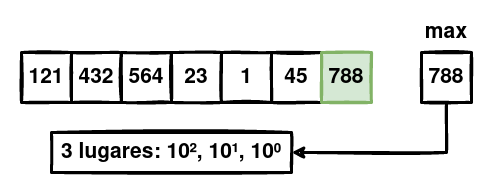
\includegraphics[width=0.75\linewidth]{images/radixsort1}
\end{center}
\end{frame}

\begin{frame}[fragile]
 \frametitle{Radix Sort: Idea General}
\begin{center}
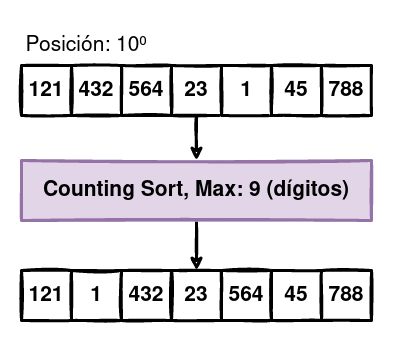
\includegraphics[width=0.75\linewidth]{images/radixsort2}
\end{center}
\end{frame}

\begin{frame}[fragile]
 \frametitle{Radix Sort: Idea General}
\begin{center}
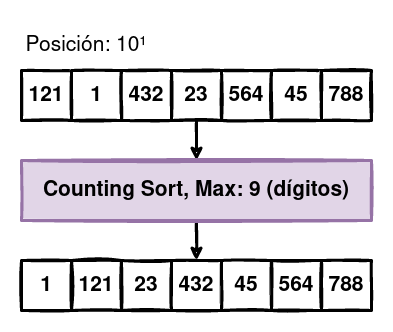
\includegraphics[width=0.75\linewidth]{images/radixsort3}
\end{center}
\end{frame}

\begin{frame}[fragile]
 \frametitle{Radix Sort: Idea General}
\begin{center}
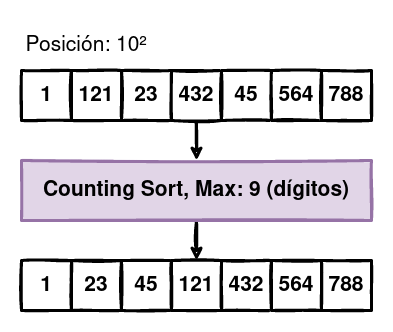
\includegraphics[width=0.75\linewidth]{images/radixsort4}
\end{center}
\end{frame}

\begin{frame}[fragile]
 \frametitle{Radix Sort}
\begin{exampleblock}{Radix Sort}
\begin{lstlisting}[language=C, basicstyle=\tiny, escapeinside={|}{|}]
int maximo(int *A, int tam) {
	int i;
	int mayor = A[0];
	for (i = 1; i < tam; i++)
		if (A[i] > mayor)
			mayor = A[i];
	return mayor;
}

void RadixSort(int *A, int tam) {
	int pos;
	int max = maximo(A, tam);

	for (pos=0 ; (max/ pow(10,pos)) > 0; pos++)
		CountingSort(A, tam, pow(10,pos));
}

\end{lstlisting}
\end{exampleblock}
\end{frame}

\begin{frame}[fragile]
 \frametitle{Radix Sort}
\begin{exampleblock}{Radix Sort: built-in Counting Sort}
\begin{lstlisting}[language=C, basicstyle=\tiny, escapeinside={|}{|}]
void CountingSort(int *A, int tam, int lugar) {
	int B[tam], i, ind_sgte, veces;
	int max = (A[0] / lugar) |\%| 10; //por si no hay digitos finales

	for (i = 1; i < tam; i++) {
		if (((A[i] / lugar) |\%| 10) > max)
			max = (A[i]/lugar)|\%| 10;
	}

	int C[max + 1];

	for (int i = 0; i < max; ++i)
		C[i] = 0;

	for (int i = 0; i < tam; i++)
		C[(A[i] / lugar) |\%| 10]++;
  
	ind_sgte = 0;
	for(i=0;i<tam;i++){ //indice siguiente
		veces=C[i];
		C[i] = ind_sgte;		
		ind_sgte += veces;
	}

	for(i=0;i<tam;i++){ //paso a B
		B[C[(A[i]/lugar) |\%| 10]] = A[i];
		C[(A[i]/lugar) |\%| 10]++;
	}

}
\end{lstlisting}
\end{exampleblock}
\end{frame}

\begin{frame}[fragile]
 \frametitle{Ejercicio}
\begin{itemize}
\item Utilizando RadixSort, ordene lexicográficamente la siguiente lista de palabras en inglés: cow, dog, sea, rug, row, mob, box, tab, bar, ear, tar, dig, big, tea, now, fox.
\end{itemize}
\end{frame}

\end{document}
